\documentclass[11pt,fleqn]{article}

\usepackage[latin1]{inputenc}
\usepackage{enumerate}
\usepackage[hang,flushmargin]{footmisc}
\usepackage{amsmath}
\usepackage{amsfonts}
\usepackage{amssymb}
\usepackage{amsthm}
\usepackage{graphicx}
\graphicspath{{images/}}
\usepackage{url}


\theoremstyle{definition}
\newtheorem{theorem}{Theorem}
\newtheorem{lemma}[theorem]{Lemma}
\newtheorem{corollary}[theorem]{Corollary}
\newtheorem{proposition}[theorem]{Proposition}
\newtheorem{definition}[theorem]{Definition}
\newtheorem{example}[theorem]{Example}

\setlength{\oddsidemargin}{0px}
\setlength{\textwidth}{460px}
\setlength{\voffset}{-1.5cm}
\setlength{\textheight}{20cm}
\setlength{\parindent}{0px}
\setlength{\parskip}{10pt}

\begin{document}
\begin{center}
{\Huge
Learning About Git
}\\
\end{center}

\section{Background}
Git is a form of version control. This means that when we control our code with git, we can easily
revert to older versions of the code and see exactly what changes were made.In addition to seeing
what changes were made, we can use git to sync our code with a cloud service. This is especially
useful since this allows us to save our code off site (on a server or something) and everything
about our code will remain the same. This makes life easy since it protects us from daily accidents
like deleting all of our code or loosing our laptop. Learning to effectively use git can be
challenging and time consuming, but it is easy to get started with the basics. 

\section{Some Stuff about OS}
As a programmer, you may often hear someone say: ``Macs are great for programming and Windows just
sucks for everything.'' I'm a fan of OSX because it really does make programming easier and life
easier in general. From one programmer to another, I would \textit{highly} recommend getting a
Macbook for your programming subteam. If getting an apple laptop is not
fiscally possible, I would recommend installing Linux on a dedicated programming laptop. Using
Windows for FTC is possible, but life is just easier on Linux or OSX.  

\section{Installing Git}
Here's the first example of why OSX and Linux is better than Windows. If you're on windows, good
luck with the installation and don't give up immediately. 

Follow the directions from here: \\
\url{https://git-scm.com/book/en/v2/Getting-Started-Installing-Git}

Next:

Install the following from GitHub and follow all the set up.\\ 
\url{https://desktop.github.com}

\section{The Idea Behind Git}
Before we jump into our first Git project, we need to learn how git works. The easiest way to
conceptualize git is by thinking of it as a tree. Take a look at this diagram:

\begin{center} 
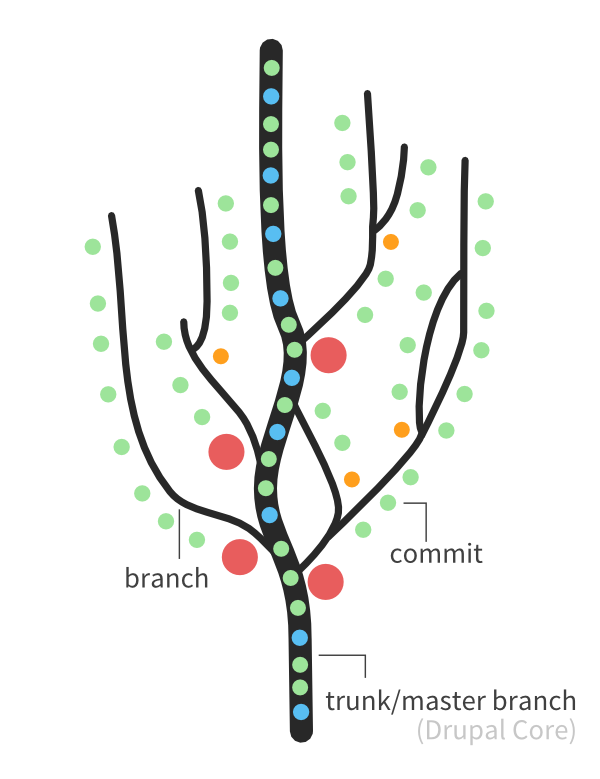
\includegraphics[scale=.5]{gitDiagram}
\end{center}

The trunk of this tree is called the master branch. In git, this means that master is the main code
that is being made. We also see that there are branches to this tree and that one particular branch
is aptly named ``branch''. This branch is coming off the master code (the trunk) and it represents a
different user's code. For example, say that I made a website template and pushed it to git. This
website template would be ``master''. Now let's say that I did a good job designing this template and you
 want to use my template to make your website. You would make a ``branch'' of my code that would
contain code that is only relevant to you. So although I made the template in master, all the
personalization you made is in a separate branch that you can edit. 

Finally, the last thing we need to talk about is a ``commit''. You can see that a commit is
represented the same way a ``branch'' in the diagram, but this is only partially true. When you
``commit'' code, you are updating the master branch and adding new code. Since git is awesome, even
though you make a commit, you can always revert back to an older version of code before you made a
specific commit. 

So now that we have a decent understanding of how git works, we can look into how to actually apply
these concepts to a project. 

\section{Learning to use Git}
   

   

\end{document}
